\chapter{ Технологический раздел}
\label{cha:technological}

    В данном разделе будут выбраны средства реплизации ПО и представлен листинг кода. 

    \section{Средства реализации}
        В данной работе используется язык программирования C++, так как
        язык позволяет написать программу, работающую относительно быстро. 
        Проект выполнен в IDE Visual Studio 2019\cite{visual-studio}

        Для замера процессорного времени была использован QueryPerformanceCounter\cite{QueryPerformanceCounter} 
        из библиотеки WinAPI.

        \begin{lstlisting}[language=C++, caption=Функция замера времени]
using funcDL = std::size_t( * )(const char*, const char* );
double getTime(funcDL getDL, const char* s1, const char* s2, int samples)
{
    LARGE_INTEGER StartingTime, EndingTime, ElapsedMicroseconds;
    LARGE_INTEGER Frequency;

    QueryPerformanceFrequency(&Frequency);
    QueryPerformanceCounter(&StartingTime);

    // Activity to be timed
    for (size_t i = 0; i < samples; i++)
        getDL(s1, s2);

    QueryPerformanceCounter(&EndingTime);
    ElapsedMicroseconds.QuadPart = EndingTime.QuadPart - StartingTime.QuadPart;

    ElapsedMicroseconds.QuadPart *= 1000000;
    ElapsedMicroseconds.QuadPart /= (Frequency.QuadPart * samples);
    return ElapsedMicroseconds.QuadPart;
}
        \end{lstlisting}

    \section{Листинг программы}
        Ниже представлены листинги кода поиска растояния Левенштейна: \begin{enumerate}
            \item нерекурсивного с заполнением матрицы (\ref{lst:matr:Levenstein});
            \item рекурсивного без заполнения матрицы (\ref{lst:rec:Levenstein});
            \item рекурсивного с заполнением матрицы (\ref{lst:rec-matr:Levenstein});
        \end{enumerate}
        
        и код функции поиска растояния Дамерау-Левенштейна (\ref{lst:matr:Dameray-Levenstein}).

        \begin{lstlisting}[language=C++, label=lst:matr:Levenstein, caption=Функция нерекурсивного поиска с заполнением матрицы]
std::size_t getLevMatr(const char* s1, const char* s2)
{
        auto n = strlen(s1);
        auto m = strlen(s2);
        auto matr = Matrix(n + 1, m + 1);

        for (size_t i = 0; i <= n; i++)
                matr[i][0] = i;

        for (size_t j = 1; j <= m; j++)
                matr[0][j] = j;

        for (size_t i = 1; i <= n; i++)
        {
                for (size_t j = 1; j <= m; j++)
                {
                        matr[i][j] = _min(_min(
                                matr[i - 1][j] + 1,
                                matr[i][j - 1] + 1),
                                matr[i - 1][j - 1] + (s1[i - 1] != s2[j - 1])
                        );
                }
        }

        return matr[n][m];
}
        \end{lstlisting}

        \begin{lstlisting}[language=C++, label=lst:rec:Levenstein, caption=Функция рекурсивного поиска без заполнения матрицы]
std::size_t getLevRec(const char* s1, const char* s2)
{
        std::size_t i = strlen(s1);
        std::size_t j = strlen(s2);
        return _getLevRec(s1, i, s2, j);
}
std::size_t _getLevRec(const char* s1, size_t i, const char* s2, size_t j)
{
	std::size_t d;
	if (i == 0)
		d = j;
	else if (j == 0)
		d = i;
	else
	{
		d = _min(_min(
			_getLevRec(s1, i, s2, j - 1) + 1,
			_getLevRec(s1, i - 1, s2, j) + 1),
			_getLevRec(s1, i - 1, s2, j - 1) + (s1[i - 1] != s2[j - 1])
		);
	}
	return d;
}
        \end{lstlisting}

        \begin{lstlisting}[language=C++, label=lst:rec-matr:Levenstein, caption=Функция рекурсивного поиска с заполнением матрицы]
std::size_t getLevRecMatr(const char* s1, const char* s2)
{
    std::size_t n = strlen(s1);
    std::size_t m = strlen(s2);
    auto matr = Matrix(n + 1, m + 1);
    for (size_t i = 0; i < n + 1; i++)
        for (size_t j = 0; j < m + 1; j++)
            matr[i][j] = -1;
    return _getLevRecMatr(s1, n, s2, m, matr);
}
std::size_t _getLevRecMatr(const char* s1, size_t i, const char* s2, size_t j, Matrix& matr)
{
	if (i == 0)
		matr[i][j] = j;
	else if (j == 0)
		matr[i][j] = i;
	else
	{
		if (matr[i][j - 1] == -1)
			matr[i][j - 1] = _getLevRecMatr(s1, i, s2, j - 1, matr);
		if (matr[i - 1][j] == -1)
			matr[i - 1][j] = _getLevRecMatr(s1, i - 1, s2, j, matr);
		if (matr[i - 1][j - 1] == -1)
			matr[i - 1][j - 1] = _getLevRecMatr(s1, i - 1, s2, j - 1, matr);
		matr[i][j] = _min(_min(matr[i][j - 1], matr[i - 1][j]) + 1, matr[i - 1][j - 1] + (s1[i - 1] != s2[j - 1]));
	}

	return matr[i][j];
}
        \end{lstlisting}

        \begin{lstlisting}[language=C++, label=lst:matr:Dameray-Levenstein, caption=Функция поиска растояния Дамерау-Левенштейна]
std::size_t getDamLevMatr(const char* s1, const char* s2)
{
    std::size_t n = strlen(s1);
    std::size_t m = strlen(s2);
    auto matr = Matrix(n + 1, m + 1);
    
    for (size_t i = 0; i <= n; i++)
        matr[i][0] = i;

    for (size_t j = 1; j <= m; j++)
        matr[0][j] = j;

    for (size_t i = 1; i <= n; i++)
    {
        for (size_t j = 1; j <= m; j++)
        {
            matr[i][j] = _min(_min(
                matr[i - 1][j] + 1,
                matr[i][j - 1] + 1),
                matr[i - 1][j - 1] + (s1[i - 1] != s2[j - 1]
            ));

            if (i > 1 && j > 1 && s1[i - 1] == s2[j - 2] && s1[i - 2] == s2[j - 1])
                matr[i][j] = _min(matr[i][j], matr[i - 2][j - 2] + 1);
        }
    }

    return matr[n][m];
}
        \end{lstlisting}
    
        
    \section{Тестирование}
        \begin{table}[]
            \begin{tabular}{|c|c|c|c|c|}
            \hline
            № & строка 1 & строка 2 & \begin{tabular}[c]{@{}c@{}}ожидаемый результат \\ (р.Л, р.Д-Л)\end{tabular} & \begin{tabular}[c]{@{}c@{}}фактический результат\\ (р.Л, р.Д-Л)\end{tabular} \\ \hline
            1 & 0        & 0        & 0, 0                                                                        & 0, 0                                                                         \\ \hline
            2 & 0        & ab       & 2, 2                                                                        & 2, 2                                                                         \\ \hline
            3 & abba     & baab     & 3, 2                                                                        & 3, 2                                                                         \\ \hline
            4 & abcd     & qwer     & 4, 4                                                                        & 4, 4                                                                         \\ \hline
            \end{tabular}
        \end{table}
        \begin{figure}[h!]
            \centering
            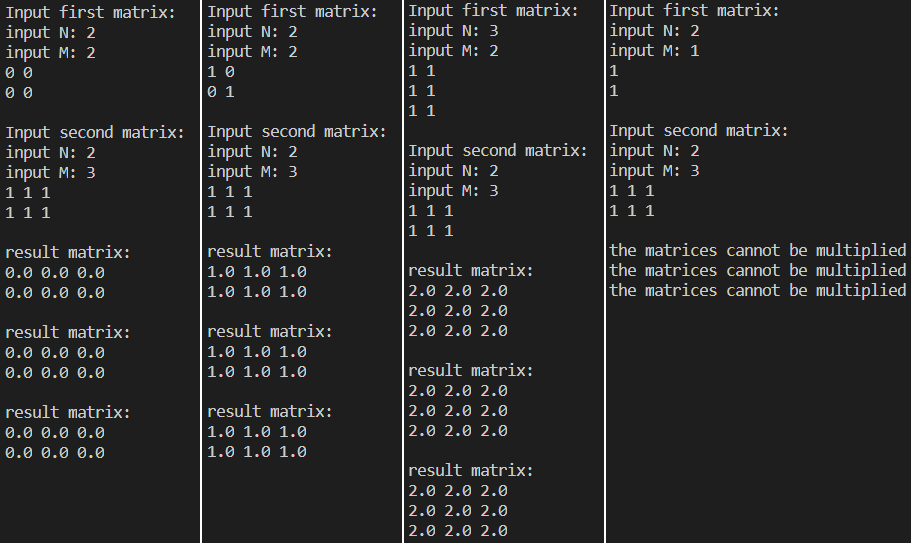
\includegraphics[scale=1.2]{testing.png}
            \caption{Результаты тестирования}
        \end{figure}

        Все тесты были пройдены.

\newpage